\section{Findings}

\subsection{Technical evaluation of the proposal's suitability}

The proposal aims to detect and report communications in which CSAM is present. In particular, the types of CSAM to be recognised are known CSAM, unknown CSAM, and child sexual solicitation (grooming).

While the proposal does not focus on the implementation details, the impact assessment accompanying the proposition presents two technical annexes. Annex 8 explains technologies covered in section \ref{ss:det_algo}. Annex 9 evaluates different approaches for CSS and SSS, introduced in section \ref{ss:scanning}.

\subsubsection{Detection of known CSAM}
\label{sss:known_csam}

To detect previously known CSAM in an E2EE communication, it is proposed in Annex 9 to use server-side scanning implementing a system similar to Microsoft's PhotoDNA but hashing the shared content on the client-side before the encryption that happens before the material is sent\cite{eu2022impact}. 

While stated in Annex 9, the proposal fails to recognize that perception hashing does not perform well in an adversarial context. 

To elaborate on this, it is possible to generate images that will trigger false positives by injecting adversarial noise in a non-CSAM image to make the hashing algorithm a hash that will collide with CSAM hash\footnote{Such an attack can be performed against Apple's Neuralhash as shown in \url{https://github.com/greentfrapp/apple-neuralhash-attack}}.

To avoid these types of attacks, the assessment aims at following a "security by obscurity" design to avoid the leaking of the algorithm. This type of design is not state-of-the-art and is not secure by design by itself\cite{SandO}. Furthermore, the algorithm will have to be run on the client side, making maintaining the secrecy of the hasher implementation difficult\footnote{See \url{https://github.com/AsuharietYgvar/AppleNeuralHash2ONNX}}.

\subsubsection{Detection of unknown CSAM}

As previously described, to detect unknown CSAM machine learning classifiers are needed. Discussing the context in which the communication is E2E encrypted, the impact assessment proposes the deployment of the classifier model on the client side and operating the classification previously the encryption of the media. Furthermore, this approach is difficult to implement, especially on smartphones and other devices with lower computational capabilities. 

Moreover, both the accompanying and the complementary impact assessment report that there exists a classifier for detecting new CSAM, Thorn's Safer, with a precision of 99.9\% and a recall of 80\%\cite{eu2022impact} \cite{eu2023impact}. Unfortunately, no proof is provided to support such claims and the citation linking to the benchmarking platform redirects to a benchmarking platform for perceptual hashing algorithms and not for classifiers of previously unknown CSAM\footnote{The link to the benchmarking platform is\\ \url{https://perception.thorn.engineering/en/latest/examples/benchmarking.html}}.

Furthermore, the performance reported in these documents is optimistic at least if compared with what has been summarized in section \ref{sss: ML}, and also taking into consideration that Thorn's model for CSAM detection is deployed on server side\cite{Thorn} having access to higher computing power.

\subsubsection{Sexual solicitation of children}

Also, in this case, ML classifiers are required to scan conversations and flag grooming behavior. Again, in E2EE communications the model must be deployed client-side. Text-based classifiers are easier to implement client-side than models based on other media as also noted in Annex 9 of the complementary impact assessment\cite{eu2022impact}. Furthermore, server-side-based solutions developed under project Arthemis are reported to have an accuracy of only 88\%\cite{eu2022impact}.

\subsubsection{Avoiding detection during CSAM sharing}
\label{sss:avoid_detection}

A simple way to avoid detection under this proposed solution is to encrypt the media before sharing it on the controlled platform. This issue is also been noted in the EDPB-EDPS Joint Opinion\cite{Joint} but never adressed in any other reviewed document.

To elaborate on this, two adversaries that aim at maintaining the file sharing anonymous could engage in a key exchange as in an insecure communication channel. Having computed a shared secret, such a secret is used to compute a symmetric key used to encrypt the media.

The following bash code and figure show how two users can share media without the system being able to detect CSAM material.
\\
\begin{minipage}{0.5\textwidth}

    \lstset{
 language=bash,
 basicstyle=\ttfamily\tiny,
 keywordstyle=\color{blue},
 commentstyle=\color{green!50!black},
 stringstyle=\color{orange},
 showstringspaces=false,
 breaklines=true,
 frame=single,
 backgroundcolor=\color{gray!10},
 captionpos=b,
 }

    \begin{lstlisting}
# Generate EC parameters for the prime256v1 (secp256v1) curve and save them to ecparam.pem
openssl ecparam -name prime256v1 -out ecparam.pem
# Generate a private key for Party 1 using the prime256v1 curve and save it to party1_private_key.pem
openssl ecparam -name prime256v1 -genkey -noout -out party1_private_key.pem
# Extract and save the public key from Party 1's private key to party1_public_key.pem
openssl ec -in party1_private_key.pem -pubout -out party1_public_key.pem
# Derive a shared secret using Party 1's private key and Party 2's public key, saving the result to shared_secret.bin
openssl pkeyutl -derive -inkey party1_private_key.pem  -peerkey party2_public_key.pem -out shared_secret.bin
# Encrypt body.bin using AES-256-CBC with the shared secret (no salt used) and save the output to body.ecb.bin
openssl enc -aes-256-cbc -nosalt -pass file:./shared_secret.bin -in body.bin -out body.ecb.bin
    \end{lstlisting}
    \captionof{lstlisting}{Client 1 exchange a secret over unsecured channel and image encryption}
\end{minipage}%
\hfill
\begin{minipage}{0.4\textwidth}
    \centering
    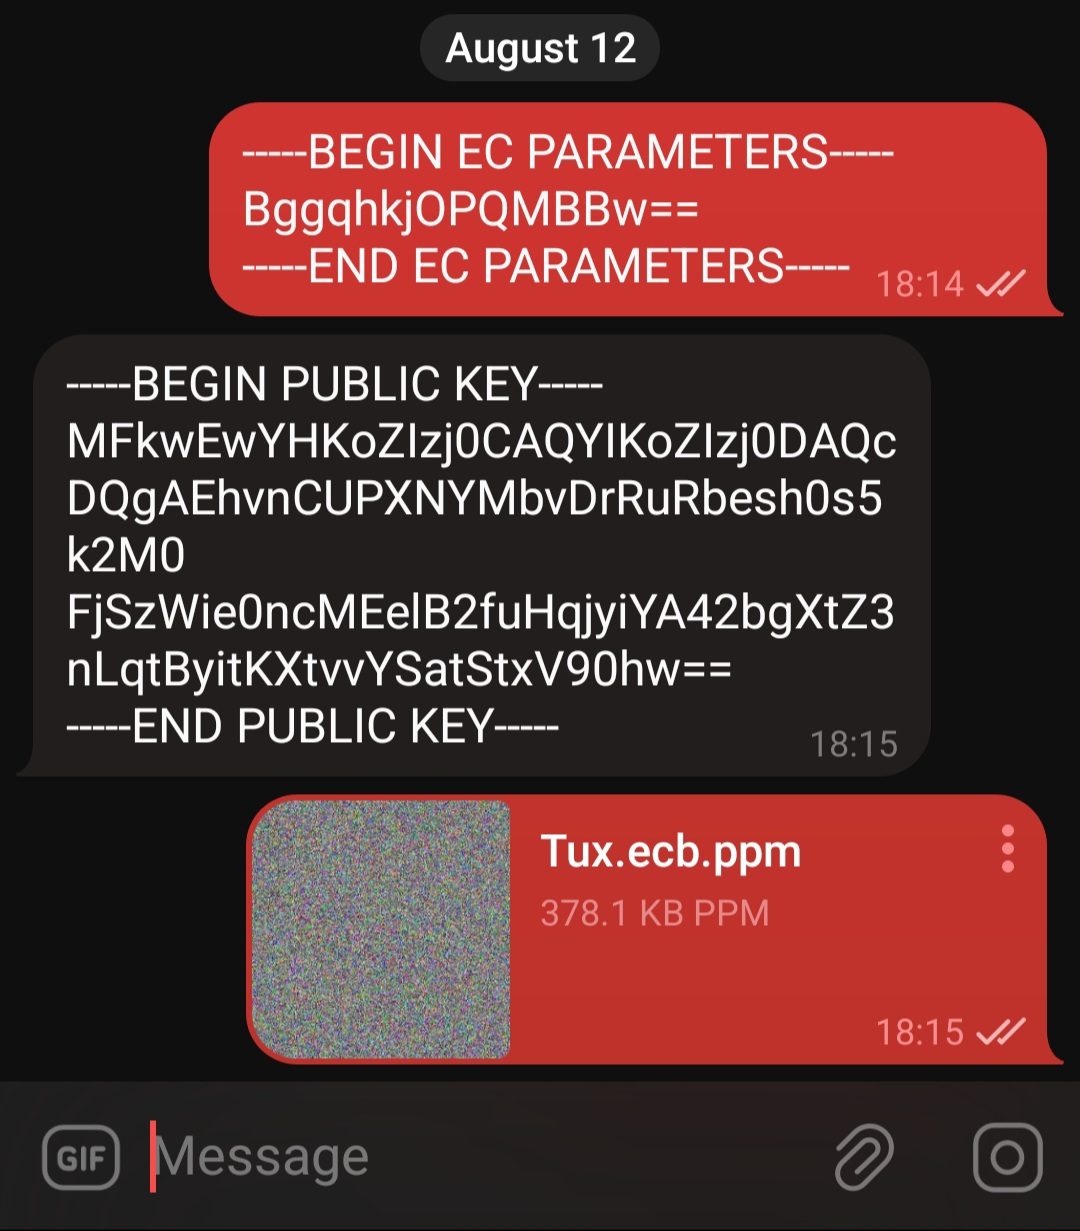
\includegraphics[keepaspectratio,width=0.85\textwidth]{05-results/img/enc_chat.jpg}
    \captionof{figure}{ECDH key exchange and AES encrypted image sharing}
\end{minipage}

\subsection{Relevant ECHR and ECJ Cases}

Following, three cases discussed by the European Court of Human Rights about mass surveillance are presented. All three cases present discussions relating to violations in Articles 8 and/or 10 of the EU Charter of Fundamental Rights.

\subsubsection{ECHR: Big Brother and others v. the United Kingdom}
\label{ss:big_brother}

As described in \cite{big_brother}, following the publication of the Snowden files that revealed the existence of an international surveillance system, the applicants complained an interference with their rights expressed by Article 8 and Article 10. The applicants claimed that their communications or communication data were tracked by the UK intelligence or obtained via service providers and/or via foreign intelligence.

The court ruled that there was indeed a violation of both Article 8 and Article 10 since secret bulk intervention was taking place. In particular, the Court defined bulk interception as a four-stage process in which (a) there is the interception and initial retention of communication data, (b) application of specific selectors to the retained data, e.g. queries, (c) examination of the selected data by analysts, (d) data retention. 

Subsequently, the Court stated that, in a lawful bulk interception, the State should clearly present the grounds upon which the interception may take place.

\subsubsection{ECHR: Breyer v. Germany}

As reported in judgment \cite{telecom}, the applicants complained that telecommunication service providers were storing their personal data outside the scope of transactions as prescribed by the Telecommunications Act (Telekommunikationsgesetz), and claimed a violation of Article 8. Such personal data were name, address, phone number, other mobile numbers, date of birth, and contract date.

The Court found that there was no violation of Article 8. More specifically, the Court notes that an interference with the applicant's privacy rights has been taking place as their personal data were being stored by the service provider. Nonetheless, the conclusion was that such interference is justified since the storage modalities, and in relation to the amount of stored data, were sufficiently clear. Furthermore, the Court accepted such interference as the measure was deemed proportional: the aim of fighting terrorism and organized crime is legitimate and the storage of the (limited and well-defined) personal data is proportionate since no sensitive data were gathered and/or processed.

\subsubsection{ECHR: Szabó and Vissy v. Hungary}

In this judgment, the applicants complained about the disproportionate and unjustified governmental policies for secret surveillance\cite{Hungary}. In particular, the applicants complained about the possibility of the system being abused. 

The court found that the scope of the measures could include virtually anyone in the interested country, with the technologies enabling the Government to intercept masses of data easily concerning even persons outside the original range of operation.

For this reason, the Court ruled that a violation of Article 8 was in place.

\subsubsection{Grand Chamber: La Quadrature du Net e a.}
\label{sss:quad}

This judicial case consists of a preliminary ruling regarding, inter alia, the interpretation of Article 15(1) of Directive 2002/58/EC (ePrivacy Directive) previously introduced in section \ref{sss:ePrivacy}.

Under the cited Article and under the consideration of articles 7, 8, and 11 of the Fundamental Right Charter, in this preliminary ruling, the Court concluded that real-time communication data collection is lawful if "recourse to automated analysis is limited to situations in which a Member State is facing a serious threat to national security which is shown to be genuine and present or foreseeable" and if "recourse to the real-time collection of traffic and location data is limited to persons in respect of whom there is a valid reason to suspect that they are involved in one way or another in terrorist activities and is subject to a prior review carried out either by a court or by an independent administrative body"\cite{Grand_chamber}.

